% ==================================================
% Batch Updates
% Author: Lester James V. Miranda
% ==================================================

\documentclass[preview, convert={outfile=\jobname-out.png,density=300}]{standalone}

\usepackage{tikz}
\usepackage{color}
\usepackage{subfig}
\usepackage{ifthen}
\usepackage{graphicx}

\renewcommand\familydefault{\sfdefault}

\usetikzlibrary{
    matrix,
    shapes,
    fit,
    arrows,
    positioning,
    calc,
    backgrounds,
    shadows.blur,
    shapes.geometric,
}

\begin{document}
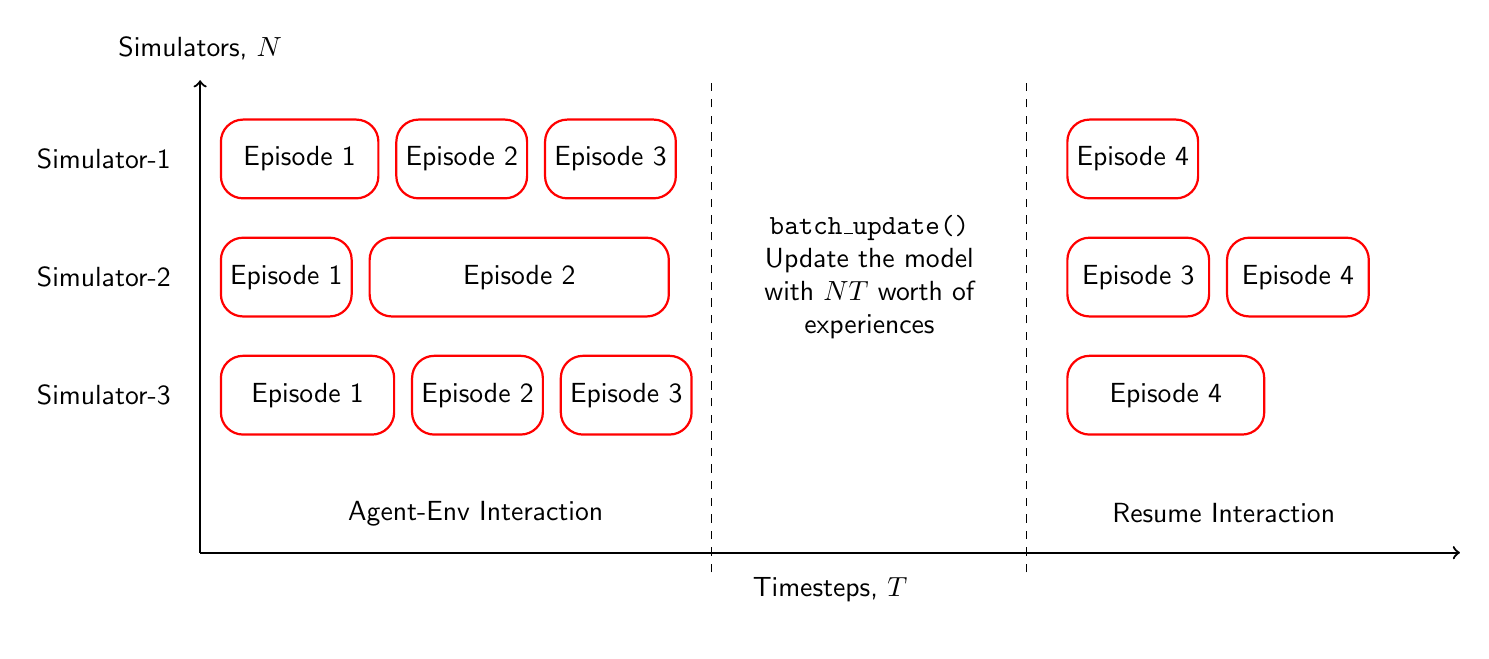
\begin{tikzpicture}[
    node distance= 0.20cm,
    episode/.style={draw, color=red, fill=none, rounded
    corners=8pt,thick, text=black, minimum width=2cm, minimum height=1cm,
anchor=west},
    textbox/.style={fill=white, align=center, minimum height=0.7cm, minimum
    width=0.7cm, anchor=east},
]

\draw[->, thick] (0,0) -- (16,0) node[label={Timesteps, $T$}, below,
    midway, yshift=-0.75cm] {};
\draw[->, thick] (0,0) -- (0,6) node[label={Simulators, $N$}] {};

% EP1
\node[episode] at (0.25,5) (ep1_1) {Episode 1};
\node[episode, minimum width=1.4cm] at (0.25, 3.5) (ep1_2) {Episode 1};
\node[episode, minimum width=2.2cm] at (0.25, 2.0) (ep1_3) {Episode 1};

% EP2
\node[episode, minimum width=1.3cm] [right=of ep1_1] (ep2_1) {Episode 2};
\node[episode, minimum width=3.8cm] [right=of ep1_2] (ep2_2) {Episode 2};
\node[episode, minimum width=1.1cm] [right=of ep1_3] (ep2_3) {Episode 2};

% EP3
\node[episode, minimum width=1.3cm] [right=of ep2_1] (ep3_1) {Episode 3};
\node[episode, minimum width=1.3cm] [right=of ep2_3] (ep3_3) {Episode 3};

% SIMULATOR LABELS
\node[textbox] at (-0.25, 5) (sim1) {Simulator-1};
\node[textbox] at (-0.25, 3.5) (sim2) {Simulator-2};
\node[textbox] at (-0.25, 2) (sim3) {Simulator-3};

% BATCH UPDATE
\draw[-, dashed] (6.5,-0.25) -- (6.5,6) {};

% TEXTBOX
\node[textbox, anchor=center] at (8.5, 3.5) (text)
    {\texttt{batch\_update()}\\Update the model\\ with $NT$
    worth of\\ experiences};

% BATCH UPDATE
\draw[-, dashed] (10.5,-0.25) -- (10.5,6) {};

% EP4
\node[episode, minimum width=1.3cm] at (11,5) (ep4_1) {Episode 4};
\node[episode, minimum width=1.8cm] at (11,3.5) (ep3_2) {Episode 3};
\node[episode, minimum width=1.8cm] [right=of ep3_2] (ep4_2) {Episode 4};
\node[episode, minimum width=2.5cm] at (11,2) (ep4_3) {Episode 4};

% TEXTBOX

\node[textbox, anchor=center] at (3.5, 0.5) (text) {Agent-Env Interaction};
\node[textbox, anchor=center] at (13.0, 0.5) (text) {Resume Interaction};

\end{tikzpicture}
\end{document}


